\documentclass[../Head/Report.tex]{subfiles}
\begin{document}
\section{Introduction}

When drones are set to fly autonomously they rely heavily on the Global Navigation System (GPS). Most of these systems comes with an error in the range of meters. To achieve better, real time kinematics (RTK) can be used, which reduces the GPS error to centimeters. However, RTK is pretty expensive and hence not an optimal solution for low cost applications. 

A solution to this problem could be to use a camera placed on the drone and analyzing the incoming data using computer vision. By placing markers on the ground, the position of these objects could be found with high precision. This would lead to autonomous flight tasks where high precision of the position is needed.      

This paper proposes methods for navigation in environments using computer vision. The basic idea of this can be seen in Figure \ref{fig:masterProjectIllustration}. Here the drone will fly autonomously using GPS coordinates until a higher accuracy is needed. In this case, it will be the navigation and precision landing of the drone using markers on the ground. Hence, the drone will follow the markers till a landing is required which is illustrated as step 3. This is a cheap and effective solution when lack of GPS precision is present e.g using low cost GPS systems or inside buildings (Hanger).

\begin{figure}[H]
	\centering
	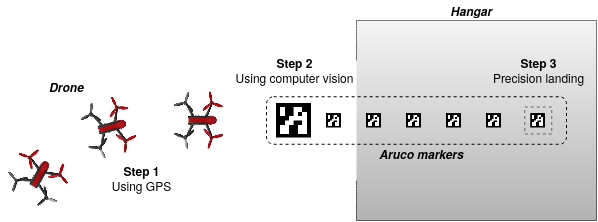
\includegraphics[height=5cm]{../Figures/masterProjectIllustration.png}
	\captionsetup{justification=centering}
    \caption{Illustration of the steps of a drone navigated autonomously using GPS to indoor navigation using computer vision leading to a precision landing }
    \label{fig:masterProjectIllustration}
\end{figure}

\begin{figure}[H]
	\centering
	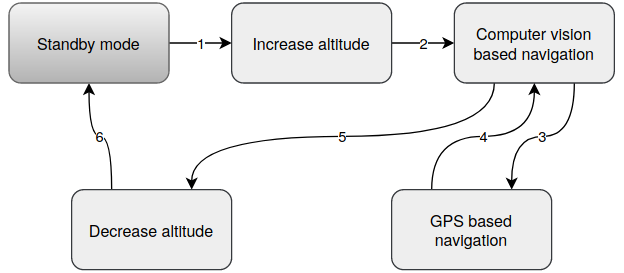
\includegraphics[height=5cm]{../Figures/simplifiedFlowchard.png}
	\captionsetup{justification=centering}
    \caption{Simplified flowchart of the autonomous flight of the drone  }
    \label{fig:simplifiedFlowchard}
\end{figure}

A simplified flowchart of this general idea can be seen in Figure \ref{fig:simplifiedFlowchard}. Here the drone must be able to fly inside a building and perform a landing using the camera data. When the drone is close enough to the marker on the ground, the GPS data will be neglected and only camera data used for navigation. This should lead to autonomous flight where the drone will be able to land and takeoff inside a building for recharging or picking up objects. However, only the precision landing will be considered in this thesis. 

In regard to the hardware used in this project, a quad-copter with a DJI SK500 frame and Pixhawk 2.1 are being considered.   



\subsection{Problem Statement}

The drone must be able to fly autonomously according to markers on the ground using computer vision. This should lead to a high precision landing where the navigation is based on the position of the markers. 

This leads to the following problems:

\begin{itemize}
    \item How can computer vision be used to detect objects?
    \item How can navigation between objects be performed?
    \item How can a precise landing be executed?
    \item How can the landing be performed in windy conditions?
    
\end{itemize} 

\subsection{Specification of requirements}

From the outline of the project as well as the problem statement, the following requirements for the project have been formulated:

\begin{itemize}
    \item The error of the landing must not exceed $\pm 10$ cm  
    \item The drone must be able to land in windy conditions e.g up to 8 m/s
    \item The landing must be performed within 5 seconds from a flying height of 2 meters 

\end{itemize}


\end{document}